\chapter{Literature Review and Related Work}
\label{chap:relatedworks}



\section{Competitor Analysis}
\label{section:competitor-analysis}

% //#TODO: place table here
% \begin{figure}[h]
%     \centering
%     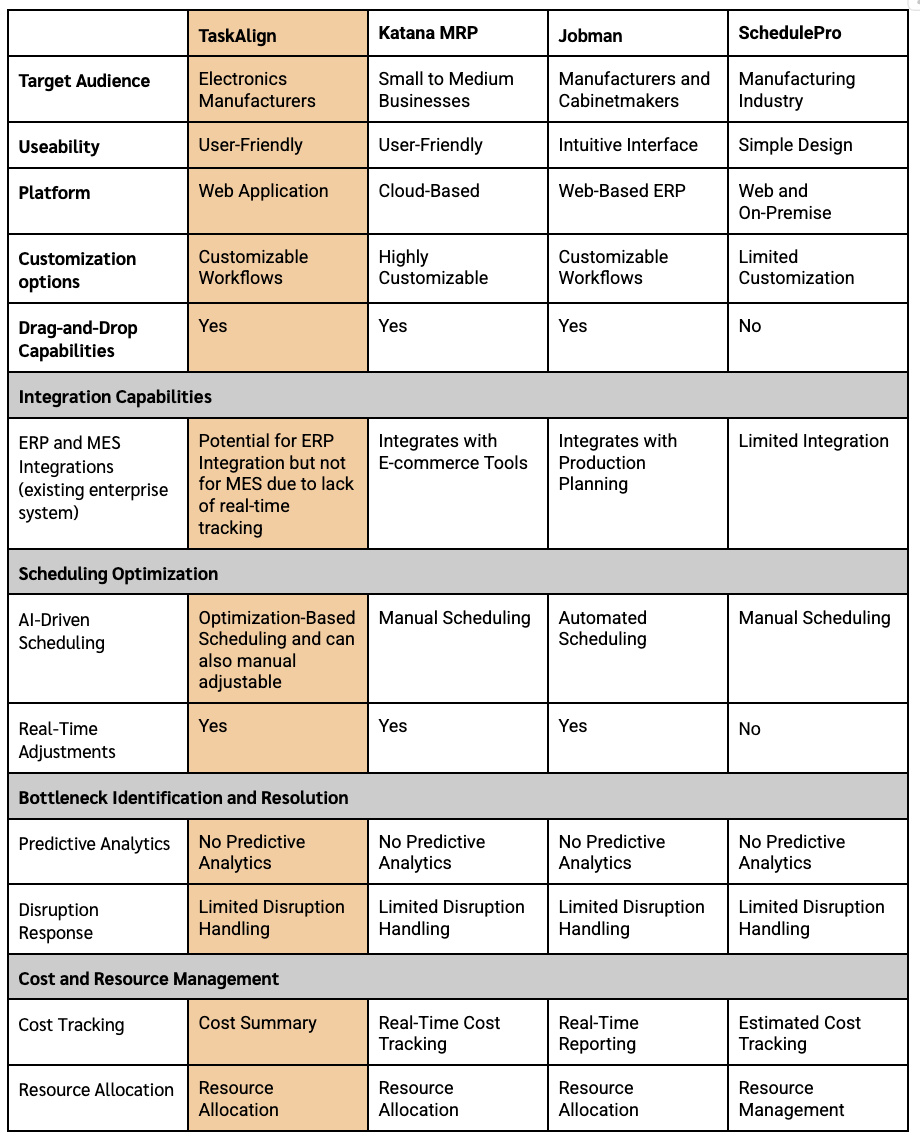
\includegraphics[width=0.5\textwidth]{examples/competitor.png}
%     \caption{Competitor Analysis Table} 
% \end{figure}

% Please add the following required packages to your document preamble:
% Beamer presentation requires \usepackage{colortbl} instead of \usepackage[table,xcdraw]{xcolor}

% Please add the following required packages to your document preamble:
% \usepackage[table,xcdraw]{xcolor}
% Beamer presentation requires \usepackage{colortbl} instead of \usepackage[table,xcdraw]{xcolor}

\begin{table}[h]
    \centering
    \renewcommand{\arraystretch}{1.3} % Adjust row height
    \setlength{\tabcolsep}{3pt} % Adjust column width
    \caption{Competitor Analysis}
    \resizebox{\textwidth}{!}{
    \begin{tabular}{|p{4cm}|p{4cm}|p{4cm}|p{4cm}|p{4cm}|}
        \hline
        & \textbf{TaskAlign} & \textbf{Katana MRP} & \textbf{Jobman} & \textbf{SchedulePro} \\
        \hline
        \textbf{Target Audience} & Electronics Manufacturers & Small to Medium Businesses & Manufacturers and Cabinetmakers & Batch and Semi-Continuous Manufacturing \\
        \hline
        \textbf{Platform} & Web Application & Cloud-Based & Web-Based ERP & Web and On-Premise \\
        \hline
        \textbf{Customization Options} & Customizable Workflows & Highly Customizable & Customizable Workflows & Limited Customization \\
        \hline
        \textbf{Drag-and-Drop Capabilities} & Yes & No Information & Yes & No \\
        \hline
        \textbf{Integration Capabilities} & ERP and MES Integrations (existing enterprise system) & Potential for ERP Integration but not for MES due to lack of real-time tracking & Integrates with E-commerce Tools & Integrates with Production Planning, Limited Integration \\
        \hline
        \textbf{Scheduling Optimization} & AI-Driven Scheduling & Optimization-Based Scheduling and can also be manually adjusted & Manual Scheduling & Automated Scheduling, Manual Scheduling \\
        \hline
        \textbf{Real-Time Adjustment} & No & Yes & Yes & No \\
        \hline
        \textbf{Bottleneck Identification and Resolution} & Predictive Analytics & No Predictive Analytics & Comes with Manufacturing Analytics & No Predictive Analytics, Statistical Analytics \\
        \hline
        \textbf{Cost and Resource Management} & Cost Tracking & Cost Summary & Real-Time Cost Tracking & Estimated Cost Tracking \\
        \hline
        \textbf{Resource Allocation} & Resource Allocation & Resource Management & Resource Allocation & Resource Management \\
        \hline
    \end{tabular}}
    \label{tab:competitor-analysis}
\end{table}


TaskAlign is a task scheduling system tailored for conventional electronics equipment factories reliant on manual production management. It empowers factory managers and operators to design optimized job schedules based on user-defined criteria, such as production time, machine utilization, and workforce allocation. The system considers constraints like machine cool-down time, energy consumption, and production dependencies. TaskAlign employs a data encoding system to translate user inputs (e.g. machine specifications, worker assignments, product requirements, dependencies) into a structured factory workflow representation suitable for optimization algorithms. These algorithms generate an optimal production schedule, maximizing machine utilization and workforce allocation while respecting constraints. Users can view and adjust schedules via Gantt charts and timelines, allowing for manual refinement of production plans. While TaskAlign does not provide real-time schedule adjustments, its optimization-based scheduling and customizable workflows offer a powerful solution for electronics manufacturers.

\subsection{Competitor Overview}

\textbf{Katana MRP}: Katana MRP is a cloud-based manufacturing ERP designed for small to medium-sized businesses. Its strengths lie in sales order fulfillment and inventory management, featuring e-commerce integration and real-time cost tracking. Katana MRP also provides manufacturing analytics and ERP and MES integrations. However, its manual scheduling approach and lack of drag-and-drop capabilities may limit its suitability for manufacturers requiring more dynamic production control \cite{katana_mrp}.

\textbf{Jobman}: Jobman is a web-based ERP solution designed for manufacturers and cabinetmakers. It includes production planning and real-time cost reporting. While Jobman offers automated scheduling and customizable workflows, it lacks predictive analytics and has limited integration capabilities, which may not fully address the needs of electronics manufacturers with complex workflows and existing enterprise systems \cite{jobman_erp}.

\textbf{SchedulePro}: SchedulePro is a scheduling software aimed at batch and semi-continuous manufacturing, offering a simple design and on-premise deployment. It provides statistical analytics and resource management features to improve production efficiency. However, its manual scheduling approach, limited customization options, and lack of integration capabilities may not meet the flexibility and connectivity needs of electronics manufacturers looking for comprehensive scheduling optimization \cite{schedulepro}.

\subsection{How TaskAlign Addresses Competitor Shortcomings}
TaskAlign distinguishes itself by catering specifically to the electronics manufacturing sector, offering optimization-based scheduling and cost summaries. Unlike Katana MRP, TaskAlign prioritizes resource allocation optimization. While Jobman provides automated scheduling, TaskAlign offers customizable scheduling tailored to electronics production, including drag-and-drop capabilities for further optimization. In contrast to SchedulePro's limited customization, TaskAlign provides highly adaptable workflows, enabling electronics manufacturers to tailor the system to their unique processes. Although TaskAlign does not offer real-time schedule adjustments, it has the potential to integrate with ERP systems, enhancing overall production management.


\section{Literature Review}
\label{section:literature-review}


\subsection{Current Approaches to Production Scheduling}

Production scheduling is a critical component of manufacturing operations that directly impacts efficiency, resource utilization, and overall productivity. Traditional production scheduling often relies heavily on human experience and manual planning, which can lead to suboptimal resource allocation and inefficiencies in complex manufacturing environments \cite{alander2024}. As manufacturing systems become increasingly complex with multiple interconnected processes, traditional scheduling methods struggle to maintain efficiency.

Chen et al. \cite{chen2023} define task scheduling as a real-time process where multiple task attributes must be considered simultaneously while different tasks are processed in parallel. This complexity is particularly evident in microservice-oriented industrial software, where multiple business processes must be executed concurrently. Their research highlights that effective scheduling must account for various characteristics, including strict real-time requirements, the coexistence of independent tasks and workflows, importance-based task attributes, and multi-task processing capabilities.

\subsection{Optimization-Based Scheduling Methods}

Optimization algorithms play a significant role in modern production scheduling approaches. Alander and Hjalmarsson \cite{alander2024} demonstrated that Genetic Algorithms (GAs) can effectively optimize production sequences, achieving up to 42\% reduction in total processing time compared to alphabetically ordered sequences. Their work emphasizes that even simple randomization of production sequences can improve efficiency by 12--17\%, highlighting the inefficiency of simplistic scheduling approaches.

Various algorithms have been developed for production scheduling optimization, including:

\begin{itemize}
    \item \textbf{First Come First Serve Algorithm (FCFS)}: Tasks are processed in order of arrival, which is simple but often inefficient.
    \item \textbf{Earliest Deadline First Algorithm (EDF)}: Prioritizes tasks with the earliest deadlines.
    \item \textbf{Least Laxity First Algorithm (LLF)}: Schedules tasks based on their laxity (deadline minus processing time).
    \item \textbf{Fixed Priority Scheduling Algorithm (FPS)}: Assigns static priorities to tasks \cite{chen2023}.
\end{itemize}

However, these traditional algorithms often fail to consider the complex constraints and multiple objectives present in modern manufacturing environments. Chen et al. \cite{chen2023} proposed a Dynamic Importance-aware Online Scheduling Algorithm (DIOS) that ranks and schedules tasks based on a comprehensive importance function considering inherent task importance, deadline constraints, and critical path factors. Their experimental results demonstrated that DIOS significantly outperformed traditional algorithms in both power system and factory production management scenarios.

\subsection{Smart Manufacturing Scheduling}

The concept of Smart Manufacturing Scheduling (SMS) represents an evolution in production scheduling, leveraging digital technologies to achieve higher levels of automation and autonomy. According to Boza et al. \cite{serranoruiz2023}, SMS integrates Digital Twin (DT) technology with Zero-Defect Manufacturing (ZDM) principles to facilitate self-managing scheduling systems that reduce or eliminate human intervention.

Digital Twin technology enables real-time simulation and optimization of manufacturing processes, allowing for dynamic adjustments in response to disruptions. This capability is particularly valuable for addressing the challenges of complex production environments with varying constraints and requirements \cite{serranoruiz2023}.

\subsection{Constraints and Resource Considerations}

Effective production scheduling must account for various constraints and resource limitations. Alander and Hjalmarsson \cite{alander2024} explored the impact of space constraints and fixtures on production efficiency, finding that optimization becomes increasingly important as resource constraints tighten. Their experiments with varying numbers of concurrent products demonstrated that scheduling efficiency is significantly affected by resource constraints, with optimization benefits becoming more pronounced under tighter constraints.

Chen et al. \cite{chen2023} introduced resource reservation and preemptive scheduling mechanisms to enhance scheduling efficiency. Their resource reservation mechanism ensures that resources needed for high-importance tasks are not allocated to lower-priority tasks, while preemptive scheduling allows urgent tasks to interrupt ongoing less critical tasks. These mechanisms were shown to improve the real-time responsiveness of scheduling systems, particularly in scenarios with time-critical tasks.

\subsection{Adaptive and Real-Time Scheduling}

Modern manufacturing environments require scheduling systems that can adapt to changing conditions and constraints. Chen et al. \cite{chen2023} incorporated an online adaptive tuning method in their DIOS algorithm to continuously adjust scheduling parameters based on real-time conditions, ensuring robust performance under dynamic manufacturing scenarios.